\documentclass[12pt]{article}
\usepackage[T1]{fontenc}
\usepackage[french]{babel}
\usepackage{datetime}
\usepackage{subcaption}
\usepackage[letterpaper, margin=1.9cm]{geometry}
\usepackage{graphicx}
\usepackage{epstopdf}
\usepackage{siunitx}
\sisetup{output-decimal-marker = {,}}
\graphicspath{ {../figures} }
\usepackage{derivative}
\usepackage{booktabs}
\usepackage[flushleft]{threeparttable}
\usepackage{amsmath}
\usepackage{parskip}

\usepackage{csquotes}
\usepackage[
backend=biber,
style=ieee,
%style=verbose,
citestyle=ieee,
%sorting=nyt,
%url=false
]{biblatex}
\bibliography{references}

\title{MEC6616 --- LAP4}


\author{Aurélie Grebe\\Noémie Herbinière}
\newdate{duedate}{19}{10}{2026}
\date{\displaydate{duedate}}

\begin{document}
\maketitle

\section{Introduction}

Dans la présente œuvre, nous proposons une résolution d'un écoulement de Couette en 2D par volumes finis. Après une brève explication de la méthode de résolution, nous analyserons les résultats à l'aide de différents maillages pour un cas de Couette classique et un cas de Couette tourné.

\section{Méthodologie}

Les équations régissant un écoulement de Couette 2D sont les suivantes:

\begin{equation} 
\frac{\partial {(\rho u u)}}{\partial x} + \frac{\partial {(\rho v u)}}{\partial y} - \mu \left(\frac{\partial^2 u}{\partial^2 x} + \frac{\partial^2 u}{\partial^2 y} \right) = - \frac{\partial P}{\partial x}
\label{eq:pde_u}
\end{equation}

\begin{equation} 
\frac{\partial {(\rho u v)}}{\partial x} + \frac{\partial {(\rho v v)}}{\partial y} - \mu \left(\frac{\partial^2 v}{\partial^2 x} + \frac{\partial^2 v}{\partial^2 y} \right) = - \frac{\partial P}{\partial y}
\label{eq:pde_v}
\end{equation}

Les équations sont exprimées en forme matricielle par: $A_u u = B_u$ et $A_v v = B_v$

Avec $A_u$ et $A_v$ contenant les coefficients de diffusion et convection, $u$ et $v$ les champs que l'on souhaite résoudre et $B_u$ et $B_v$ contenant les termes de source (ici gradient de pression) et de cross-diffusion.

\subsection{Méthode itérative}

Afin de linéariser l'équation, on définit:
$F_{x,i} = \rho u_i$ $F_{y,i} = \rho v_i$ tels des flux sur l'arrête i que l'on recalcule à chaque nouvelle itération à l'aide des u et v obtenus à l'itération précédente.

Les vitesses étant obtenus au centre de chaque élément, on approxime les $F_i$ aux arrêtes avec la moyenne suivante:
\begin{align}
F_{x,i} &= \frac{F_{x,Tg} + F_{x,Td}}{2} \\
F_{y,i} &= \frac{F_{y,Tg} + F_{y,Td}}{2} \\
F_i &= (F_{x,i} \hat{n}_{x,i} + F_{y,i} \hat{n}_{y,i}) \Delta A_i
\end{align}

Les équations du moment deviennent ainsi, à l'itération $j+1$:
\begin{align}
\frac{\partial {(F_x^j u^{j+1})}}{\partial x} + \frac{\partial {(F_y^j u^{j+1})}}{\partial y} - \mu \left(\frac{\partial^2 u^{j+1}}{\partial^2 x} + \frac{\partial^2 u^{j+1}}{\partial^2 y} \right) &= - \frac{\partial P}{\partial x} \\
\frac{\partial {(F_x^j v^{j+1})}}{\partial x} + \frac{\partial {(F_y^j v^{j+1})}}{\partial y} - \mu \left(\frac{\partial^2 v^{j+1}}{\partial^2 x} + \frac{\partial^2 v^{j+1}}{\partial^2 y} \right) &= - \frac{\partial P}{\partial y}
\end{align}

Pour un élément P, les termes sources sont $SGF_x = - \left(\frac{\partial P}{\partial x}\right)_P \Delta V_p$ et $SGF_y = - \left(\frac{\partial P}{\partial y}\right)_P \Delta V_p$.

On définit les conditions initiales pour $i=0$: $u^0=f(x,y)$ et $v^0=g(x,y)$; $F_x^0 = \rho u^0$ et $F_y^0 = \rho v^0$.

Ainsi il ne reste plus qu'à résoudre les deux équations à l'aide du solveur convection-diffusion développé dans le TPP2.

Afin de stabiliser le système, on applique une sous-relaxation:
\begin{align}
u^{j+1} &= \alpha u_P + (1-\alpha)u^j \\
v^{j+1} &= \alpha v_P + (1-\alpha)v^j
\end{align}

Où: 
$0.5<\alpha<1$, $u_P$ et $v_p$ sont les solutions respectives de $A_u^j u_P = B_u$ et $A_v^j v_P = B_v$, $u^j$ et $v^j$ sont les solutions de l'itération précédente, et $u^{j+1}$ et $v^{j+1}$ sont les solutions qui seront utilisées pour calculer les flux de la prochaine itération.

Le processus itératif continue jusqu'à la convergence de la solution. La convergence est mesurée en comparant la norme des résidus, tel que présenté ci-dessous:
\begin{align}
|A_u^{j+1} u^{j+1} - B_u| = |R_u^{j+1}| \\
|A_v^{j+1} v^{j+1} - B_v| = |R_v^{j+1}|
\end{align}


\subsection{Maillages et conditions limites}

Les maillages utilisés sont présentés en figure XXX, de taille 1x1, après avoir étudié la convergence de la solution, le nombre d'éléments choisi est de 20. 

Les conditions aux frontières pour les vitesses sont: Neumann nul sur les faces Est et Ouest, Dirichlet nul sur la face Sud (paroi fixe, no slip wall) et Dirichlet $u = U$ où $U$ est une vitesse constante appliquée sur la face Nord.


\section{Résultats}


\subsection{Couette classique}

On pose:
$\frac{\partial P}{\partial x} = -2P$ et $\frac{\partial P}{\partial y} = 0$. Ainsi, $P(x) = -2Px$.

La solution analytique correspondante est: $u = y*(1-P*(1-y))$ et $v=0$.

En faisant varier le paramètre $P = [0, 1, -3]$, on obtient les résultats suivants.

\begin{figure}
	\begin{subfigure}[t]{0.3\textwidth}
		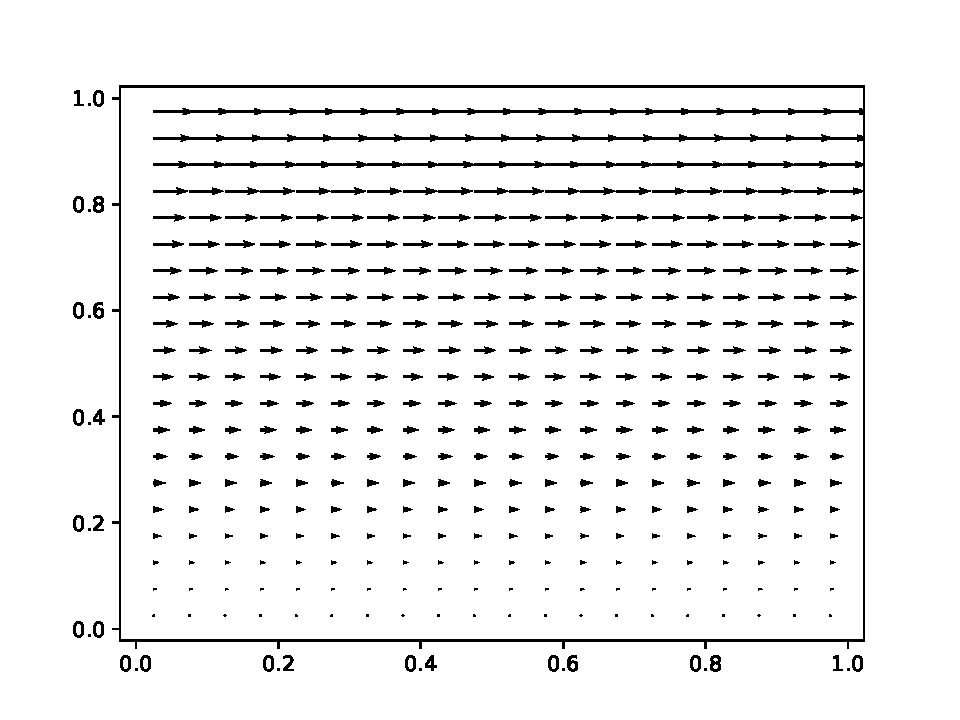
\includegraphics[width=\textwidth]{../figures/couette_vec_quad_nocd_theta_0_P_0.pdf}
		\caption{Champ vectoriel de vitesses}
	\end{subfigure}
	\hfill
	\begin{subfigure}[t]{0.3\textwidth}
		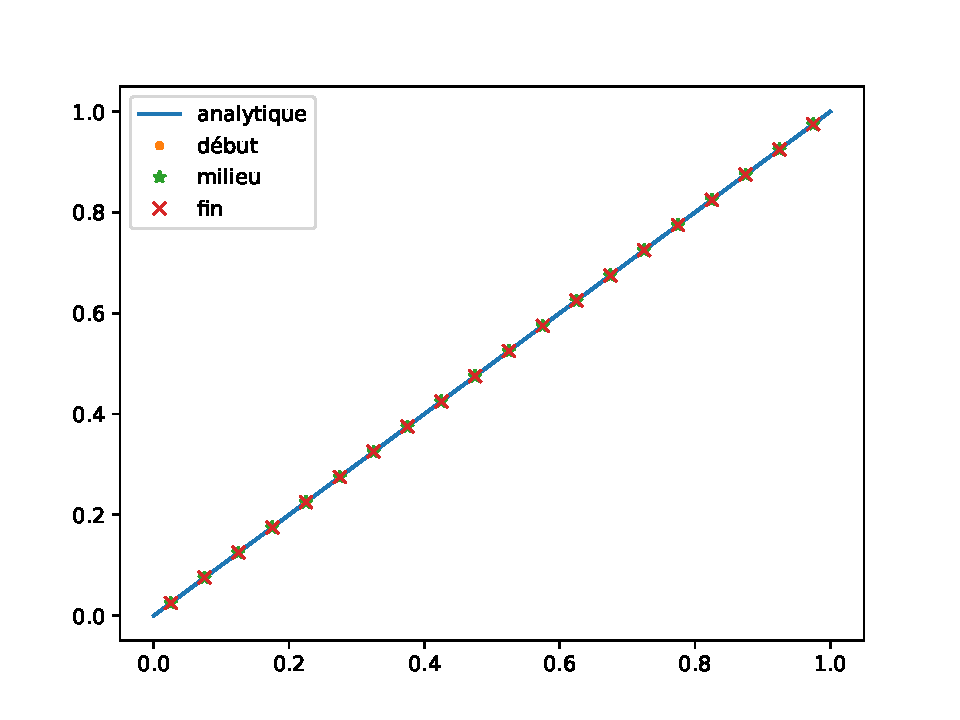
\includegraphics[width=\textwidth]{../figures/couette_slice_quad_nocd_theta_0_P_0.pdf}
		\caption{Slices de la solution numérique vs solution analytique}
	\end{subfigure}
	\hfill
	\begin{subfigure}[t]{0.3\textwidth}
		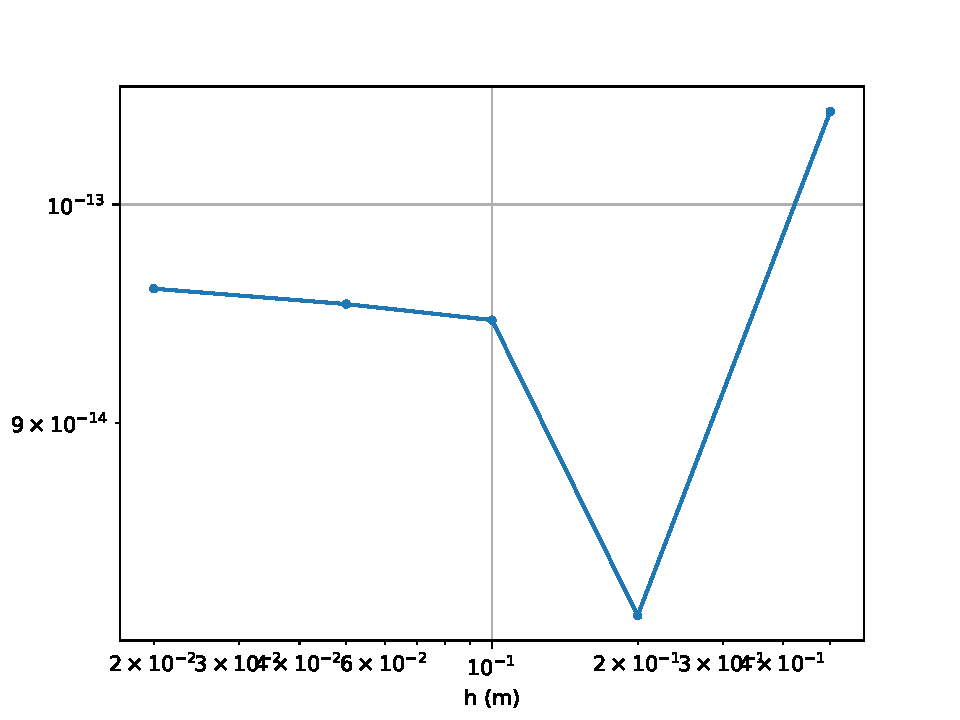
\includegraphics[width=\textwidth]{../figures/couette_err_quad_nocd_theta_0_P_0.pdf}
		\caption{Convergence}
	\end{subfigure}
	\caption{Couette classique pour P = 0 en maillage quadrilatère}
	\label{classique_p_0_quad}
\end{figure}

On observe en figure~\ref{classique_p_0_quad} que la convergence ne dépend que des erreurs de flottants car le résultat est linéaire.

\begin{figure}
	\begin{subfigure}[t]{0.3\textwidth}
		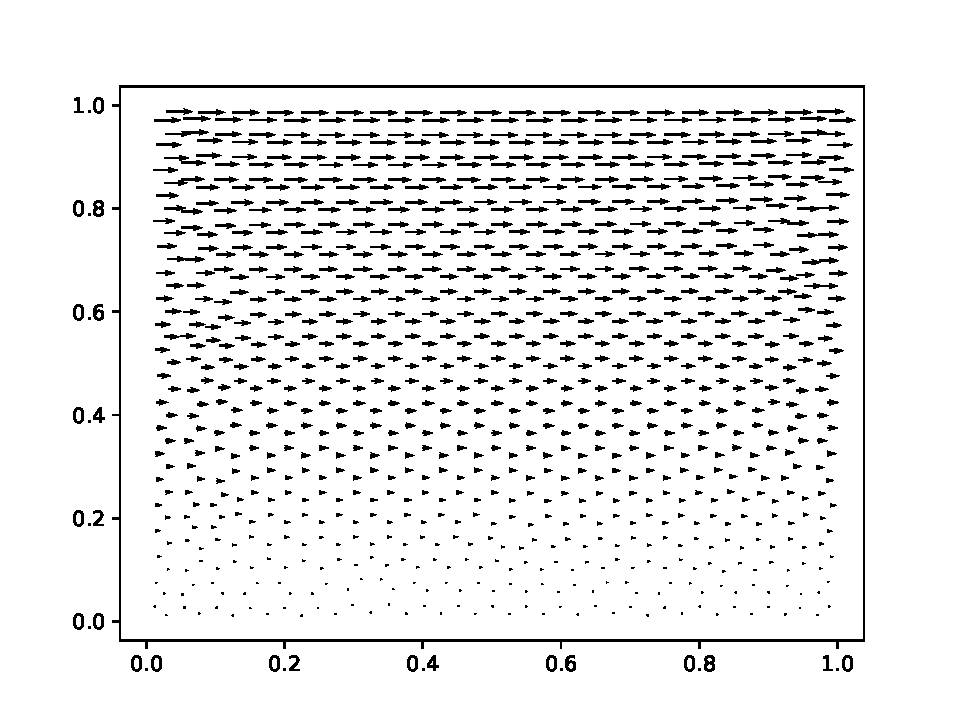
\includegraphics[width=\textwidth]{../figures/couette_vec_tri_cd_theta_0_P_0.pdf}
		\caption{Champ vectoriel de vitesses}
	\end{subfigure}
	\hfill
	\begin{subfigure}[t]{0.3\textwidth}
		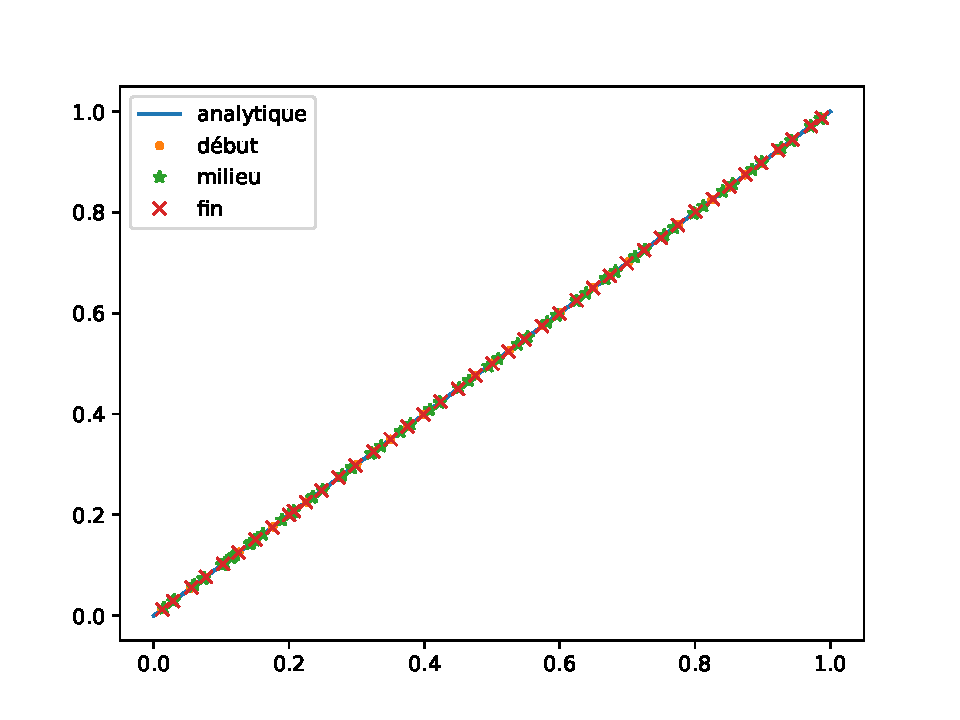
\includegraphics[width=\textwidth]{../figures/couette_slice_tri_cd_theta_0_P_0.pdf}
		\caption{Slices de la solution numérique vs solution analytique}
	\end{subfigure}
	\hfill
	\begin{subfigure}[t]{0.3\textwidth}
		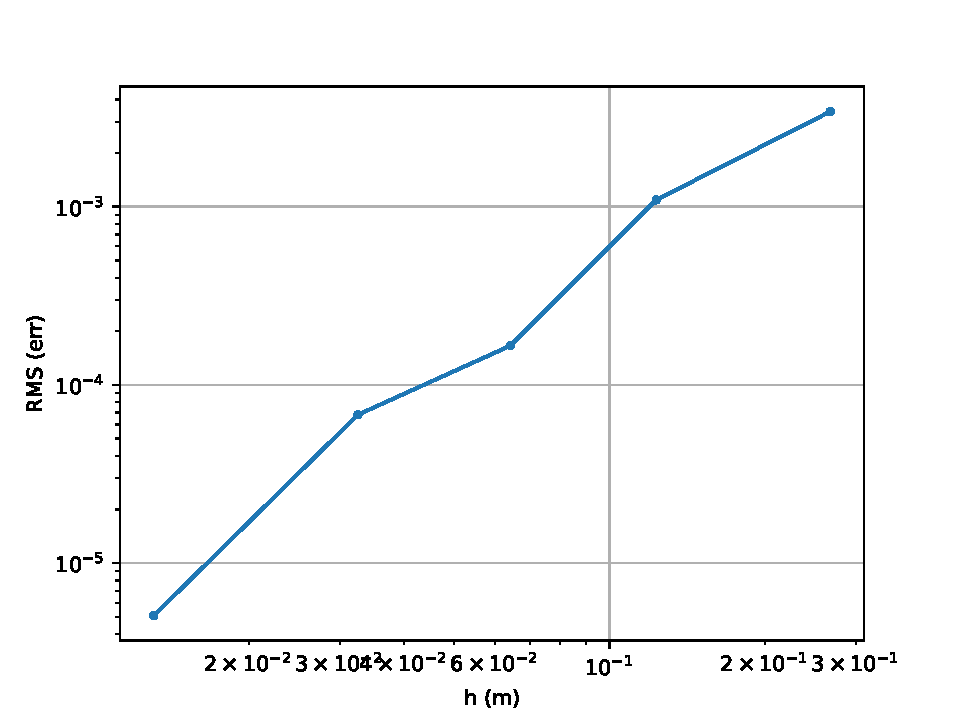
\includegraphics[width=\textwidth]{../figures/couette_err_tri_cd_theta_0_P_0.pdf}
		\caption{Convergence}
	\end{subfigure}
	\caption{Couette classique pour P = 0 en maillage triangulaire}
\end{figure}

\begin{figure}
	\begin{subfigure}[t]{0.3\textwidth}
		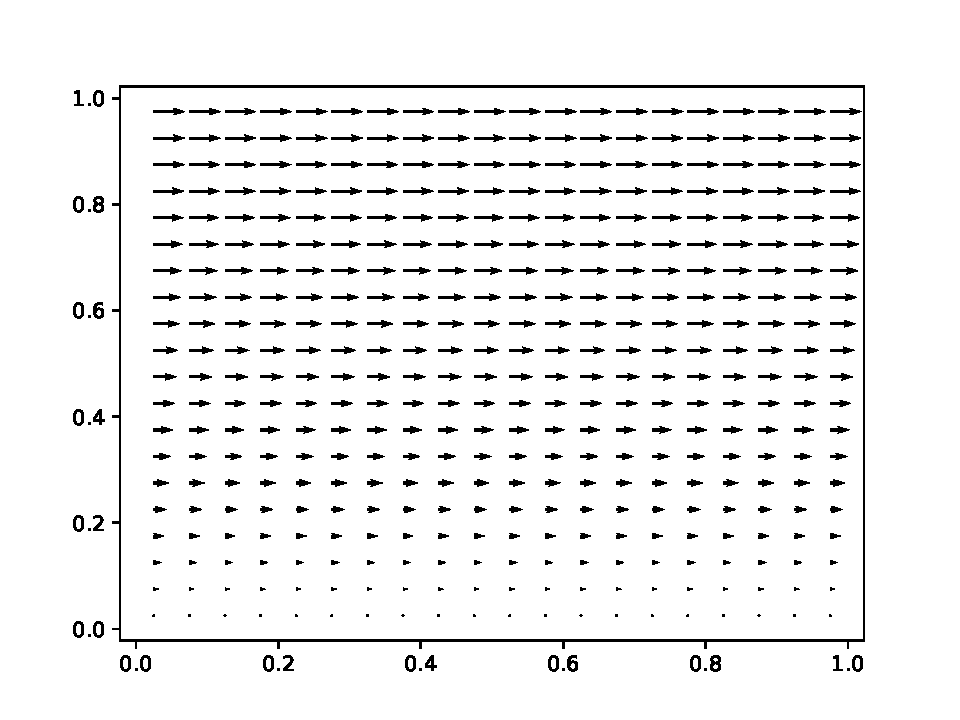
\includegraphics[width=\textwidth]{../figures/couette_vec_quad_nocd_theta_0_P_1.pdf}
		\caption{Champ vectoriel de vitesses}
	\end{subfigure}
	\hfill
	\begin{subfigure}[t]{0.3\textwidth}
		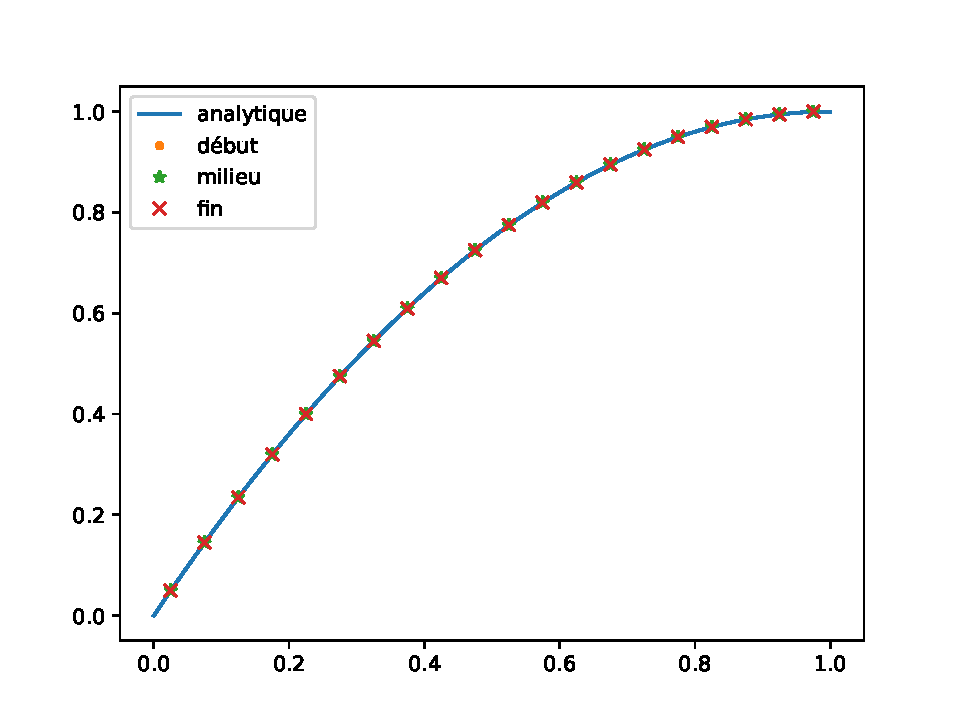
\includegraphics[width=\textwidth]{../figures/couette_slice_quad_nocd_theta_0_P_1.pdf}
		\caption{Slices de la solution numérique vs solution analytique}
	\end{subfigure}
	\hfill
	\begin{subfigure}[t]{0.3\textwidth}
		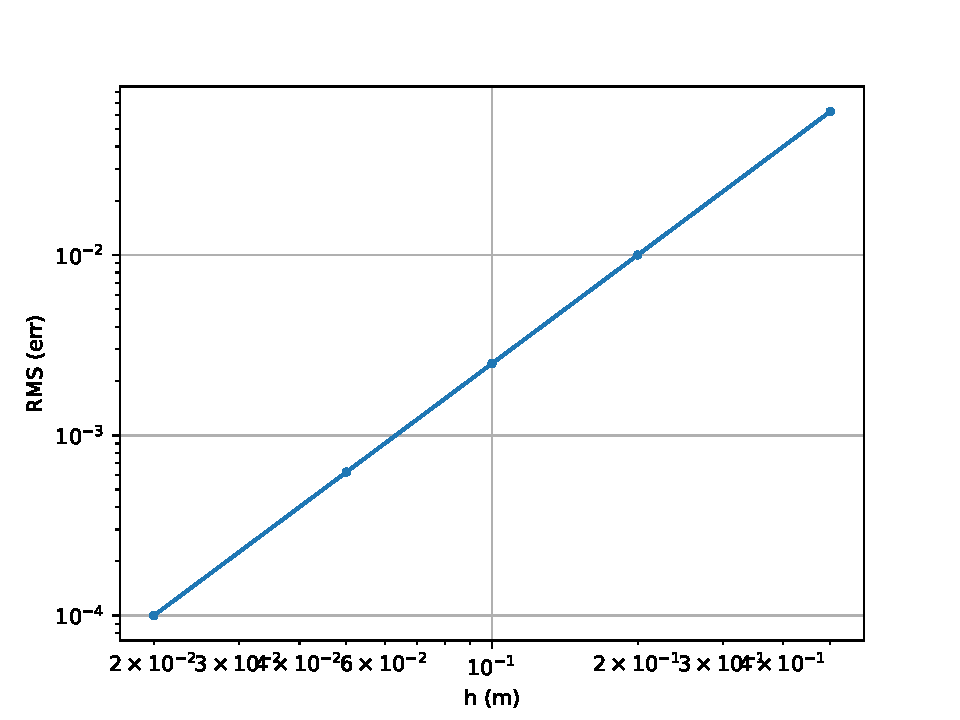
\includegraphics[width=\textwidth]{../figures/couette_err_quad_nocd_theta_0_P_1.pdf}
		\caption{Convergence}
	\end{subfigure}
	\caption{Couette classique pour P = 1 en maillage quadrilatère}
\end{figure}

\begin{figure}
	\begin{subfigure}[t]{0.3\textwidth}
		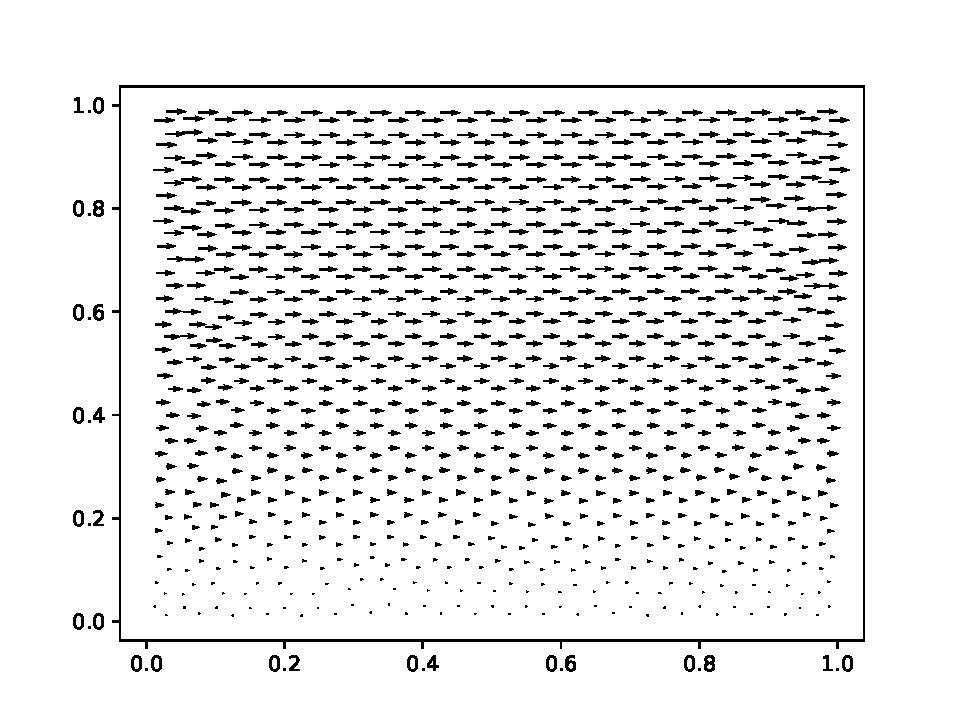
\includegraphics[width=\textwidth]{../figures/couette_vec_tri_cd_theta_0_P_1.pdf}
		\caption{Champ vectoriel de vitesses}
	\end{subfigure}
	\hfill
	\begin{subfigure}[t]{0.3\textwidth}
		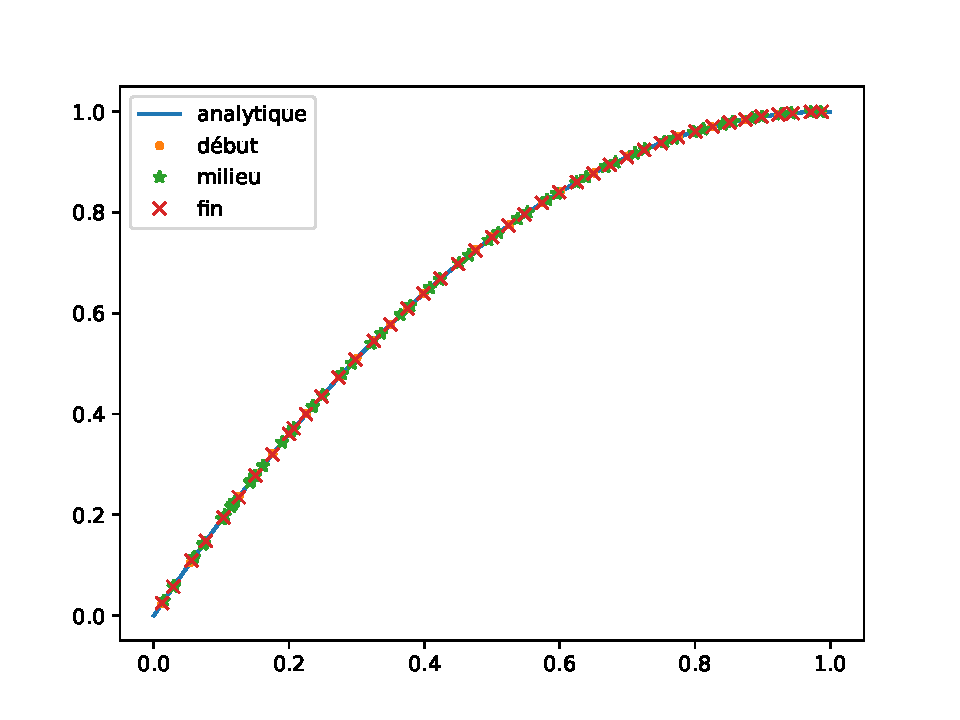
\includegraphics[width=\textwidth]{../figures/couette_slice_tri_cd_theta_0_P_1.pdf}
		\caption{Slices de la solution numérique vs solution analytique}
	\end{subfigure}
	\hfill
	\begin{subfigure}[t]{0.3\textwidth}
		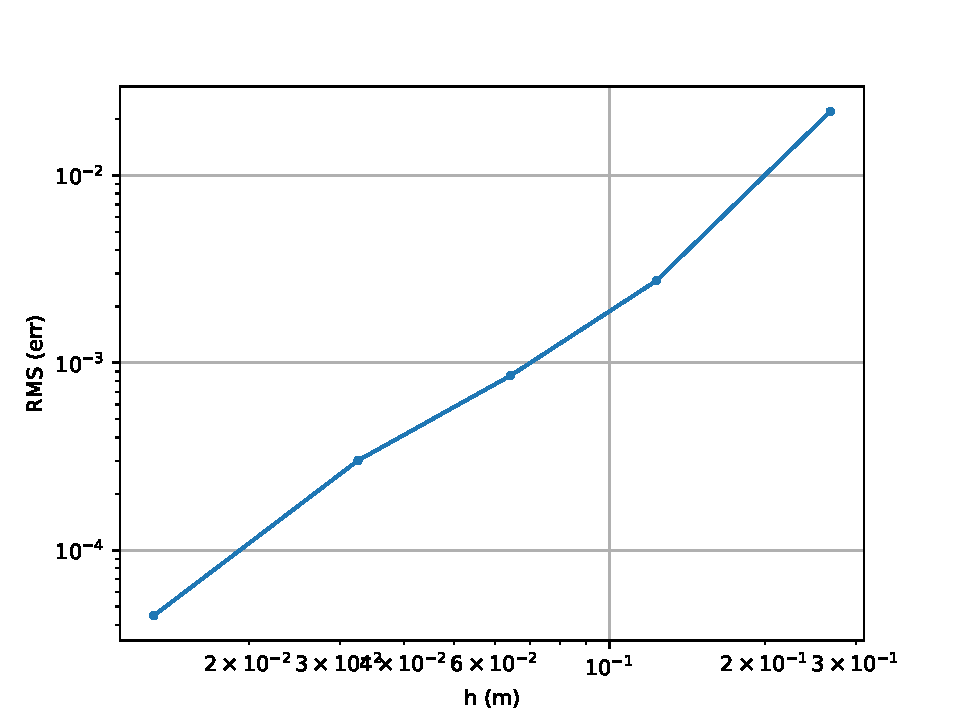
\includegraphics[width=\textwidth]{../figures/couette_err_tri_cd_theta_0_P_1.pdf}
		\caption{Convergence}
	\end{subfigure}
	\caption{Couette classique pour P = 1 en maillage triangulaire}
\end{figure}

\begin{figure}
	\begin{subfigure}[t]{0.3\textwidth}
		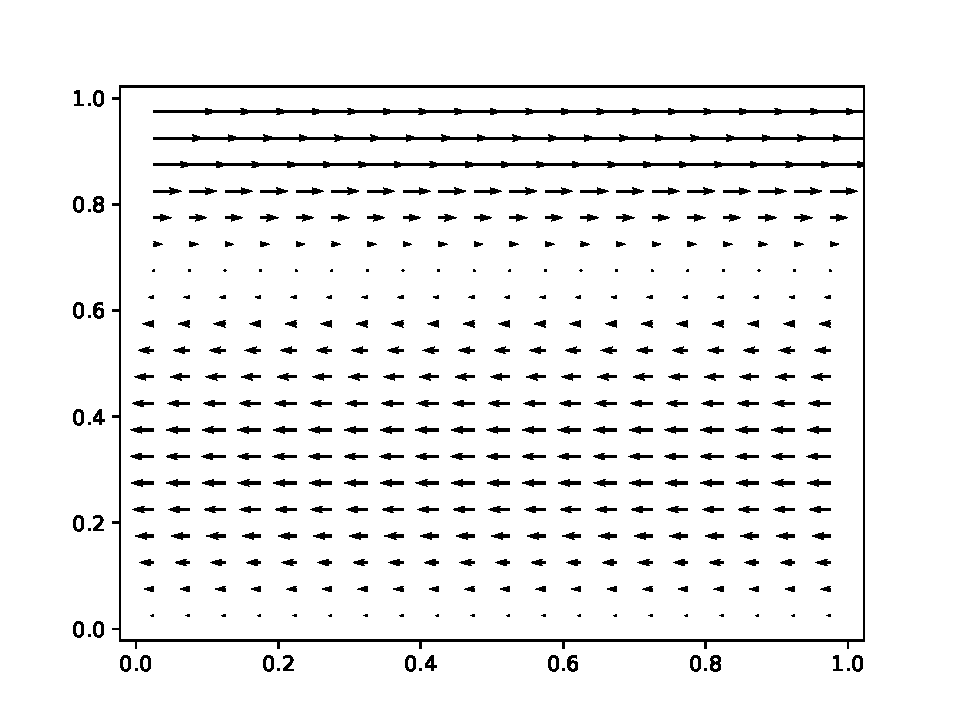
\includegraphics[width=\textwidth]{../figures/couette_vec_quad_nocd_theta_0_P_-3.pdf}
		\caption{Champ vectoriel de vitesses}
	\end{subfigure}
	\hfill
	\begin{subfigure}[t]{0.3\textwidth}
		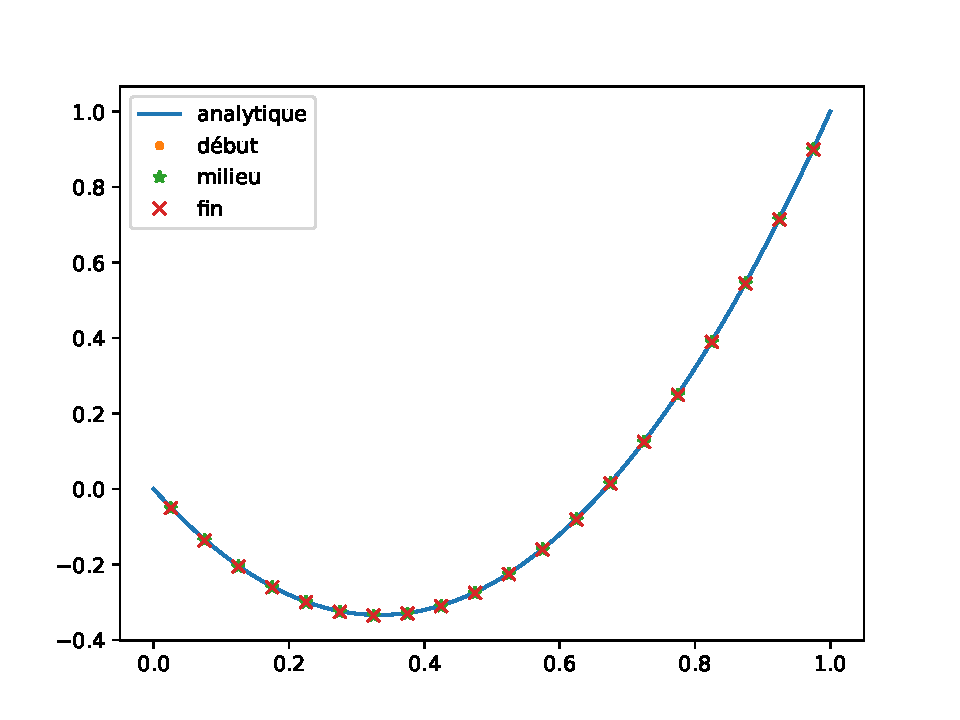
\includegraphics[width=\textwidth]{../figures/couette_slice_quad_nocd_theta_0_P_-3.pdf}
		\caption{Slices de la solution numérique vs solution analytique}
	\end{subfigure}
	\hfill
	\begin{subfigure}[t]{0.3\textwidth}
		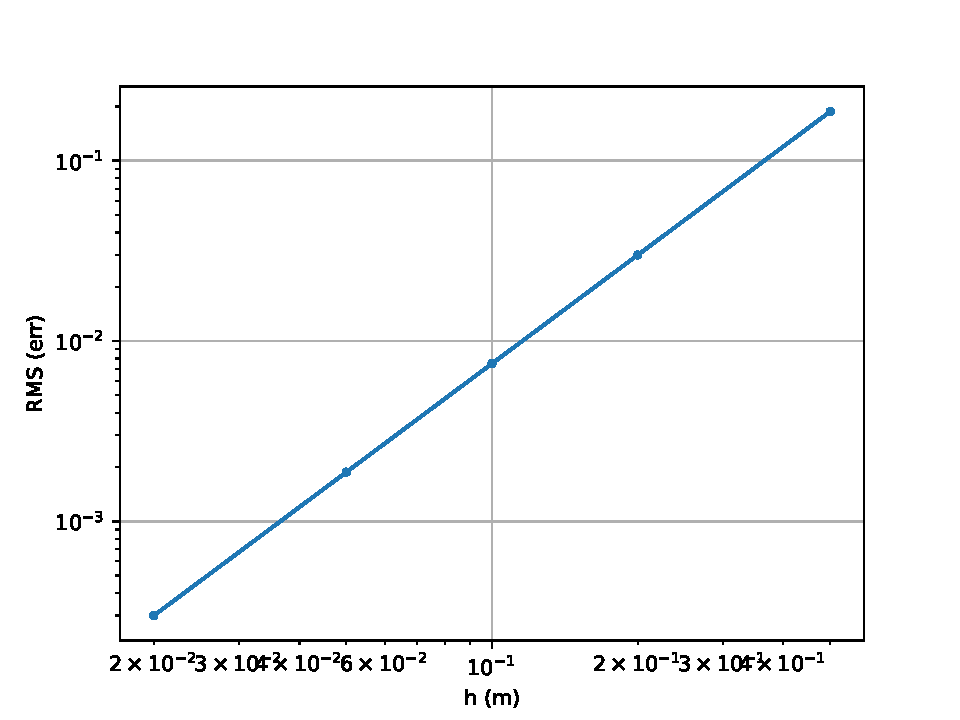
\includegraphics[width=\textwidth]{../figures/couette_err_quad_nocd_theta_0_P_-3.pdf}
		\caption{Convergence}
	\end{subfigure}
	\caption{Couette classique pour P = -3 en maillage quadrilatère}
\end{figure}

\begin{figure}
	\begin{subfigure}[t]{0.3\textwidth}
		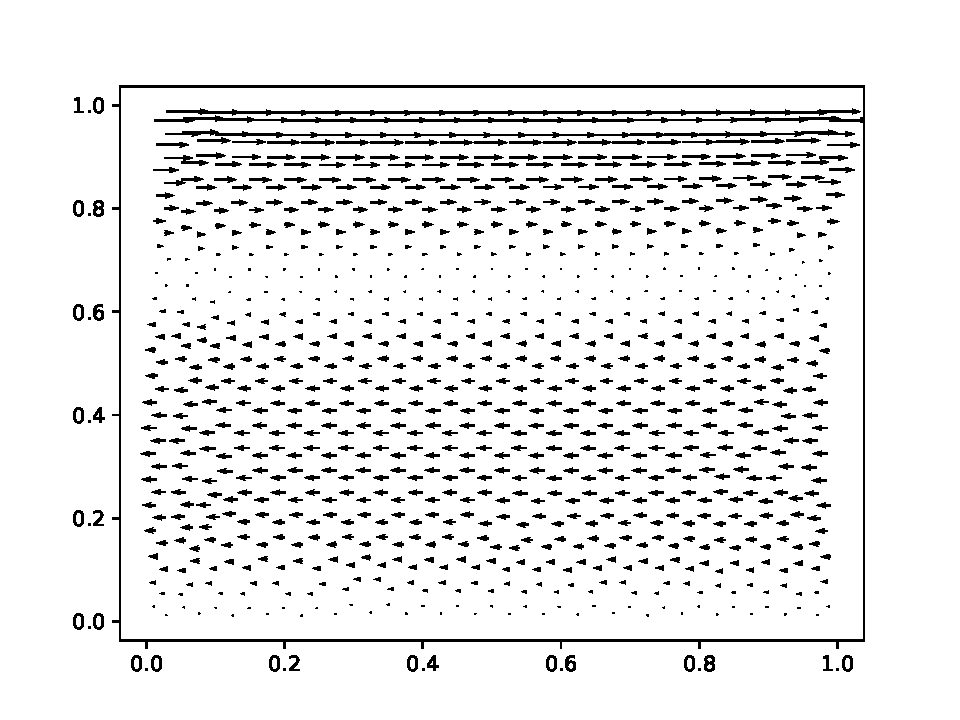
\includegraphics[width=\textwidth]{../figures/couette_vec_tri_cd_theta_0_P_-3.pdf}
		\caption{Champ vectoriel de vitesses}
	\end{subfigure}
	\hfill
	\begin{subfigure}[t]{0.3\textwidth}
		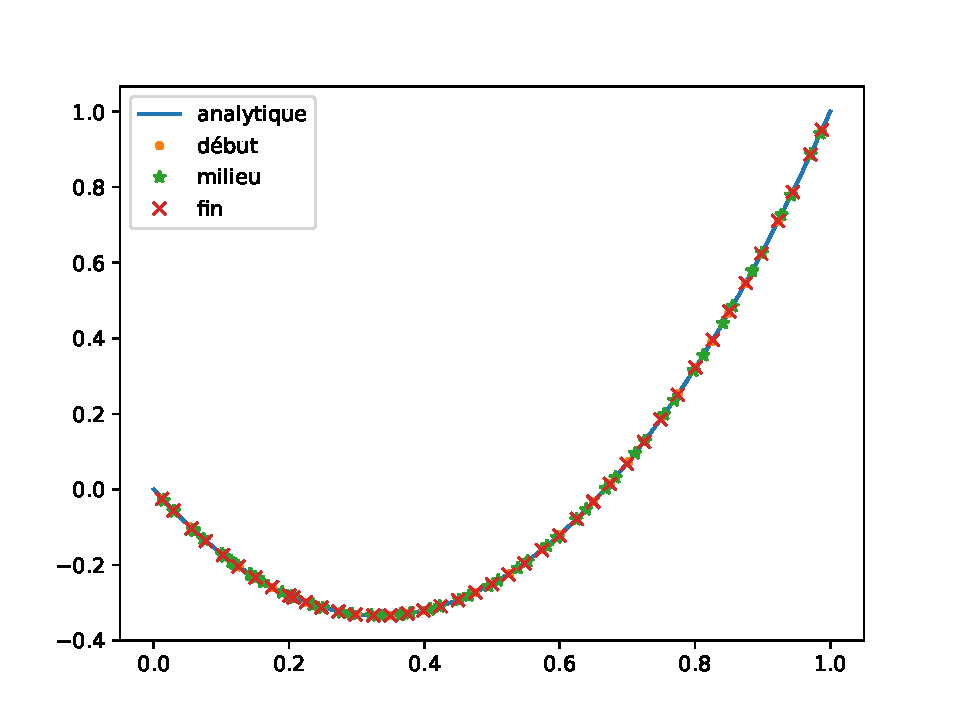
\includegraphics[width=\textwidth]{../figures/couette_slice_tri_cd_theta_0_P_-3.pdf}
		\caption{Slices de la solution numérique vs solution analytique}
	\end{subfigure}
	\hfill
	\begin{subfigure}[t]{0.3\textwidth}
		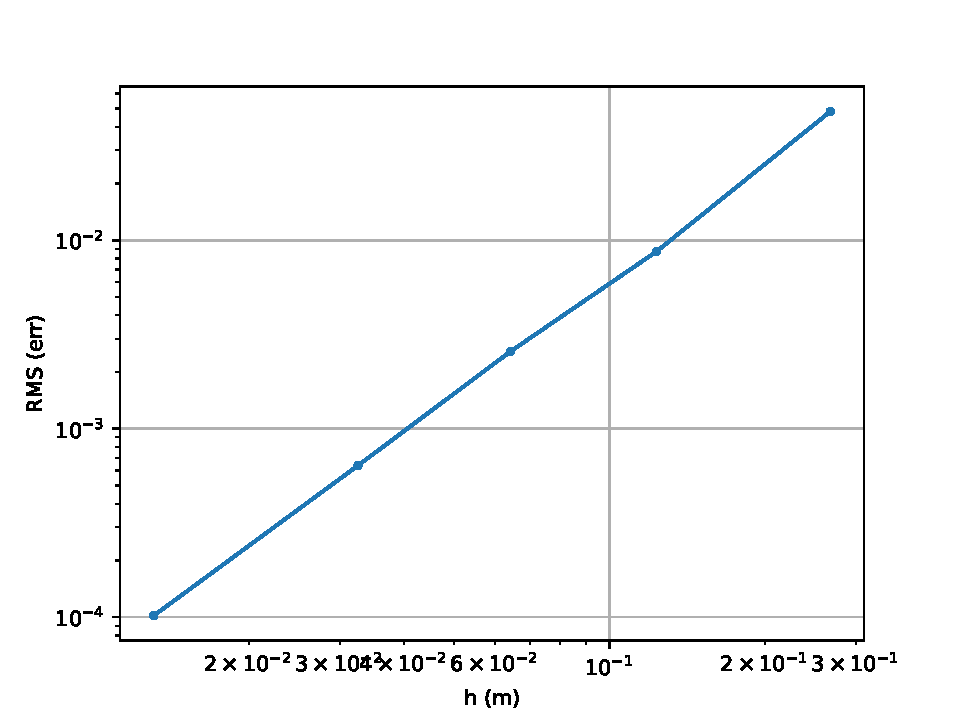
\includegraphics[width=\textwidth]{../figures/couette_err_tri_cd_theta_0_P_-3.pdf}
		\caption{Convergence}
	\end{subfigure}
	\caption{Couette classique pour P = -3 en maillage triangulaire}
\end{figure}


\subsection{Couette incliné}

Pour le cas de couette incliné, il suffit d'introduire une matrice de rotation R telle que présentée dans l'énoncé et de remplacer les coordonnées du maillage par celles multipliées par la matrice R.

On a choisi $\theta = 0.5 rad$.

On fait encore une fois varier le paramètre P et on obtient les figures suivantes.

\begin{figure}
	\begin{subfigure}[t]{0.3\textwidth}
		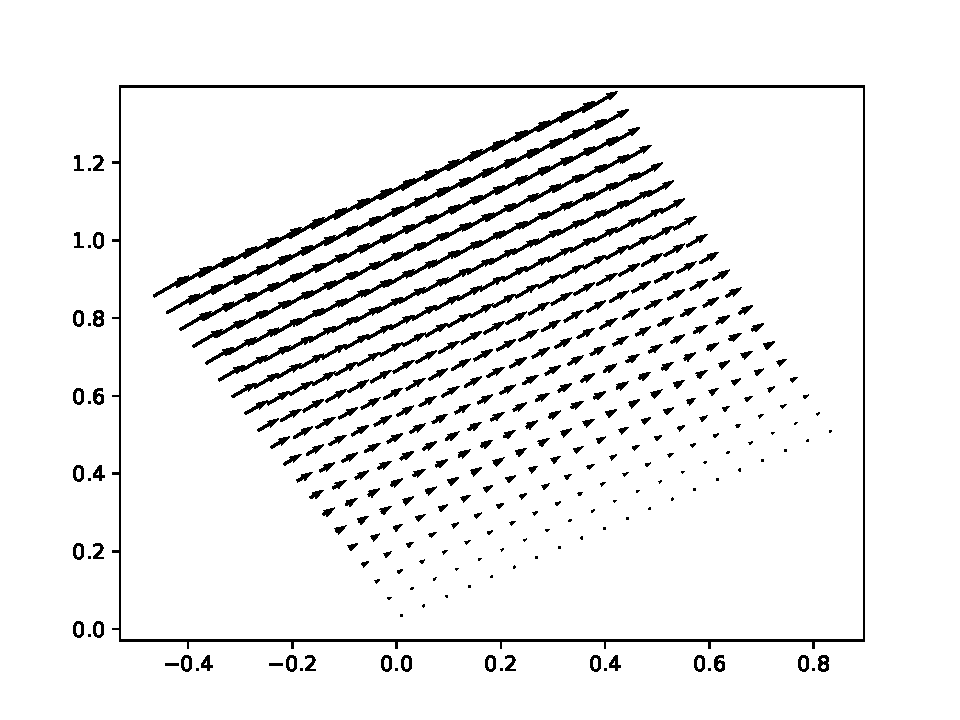
\includegraphics[width=\textwidth]{../figures/couette_vec_quad_nocd_theta_0.5235987755982988_P_0.pdf}
		\caption{Champ vectoriel de vitesses}
	\end{subfigure}
	\hfill
	\begin{subfigure}[t]{0.3\textwidth}
		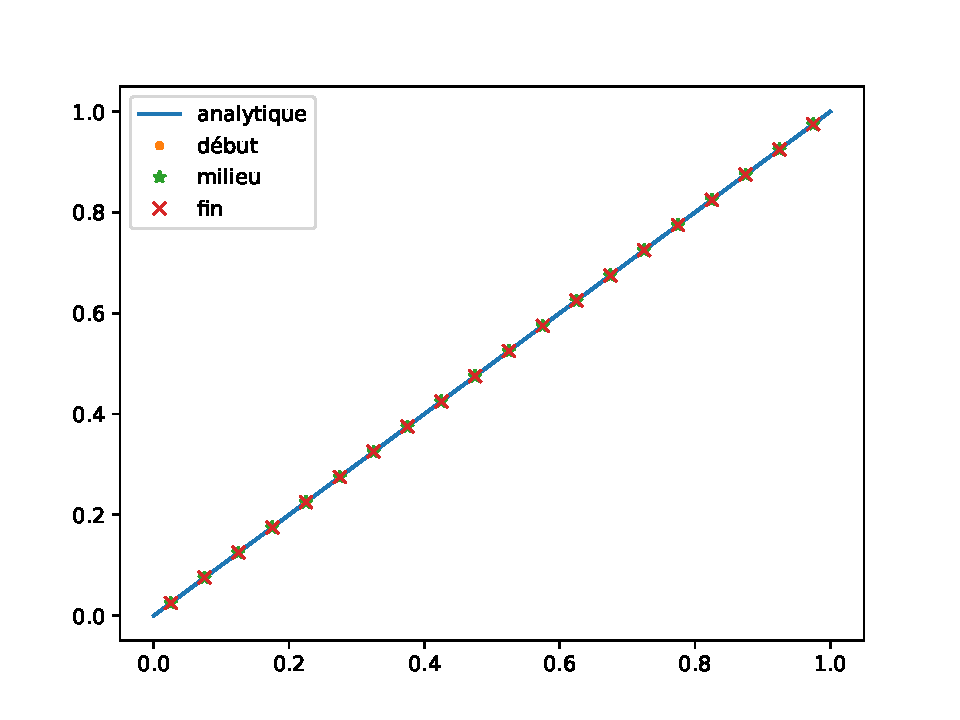
\includegraphics[width=\textwidth]{../figures/couette_slice_quad_nocd_theta_0.5235987755982988_P_0.pdf}
		\caption{Slices de la solution numérique vs solution analytique}
	\end{subfigure}
	\hfill
	\begin{subfigure}[t]{0.3\textwidth}
		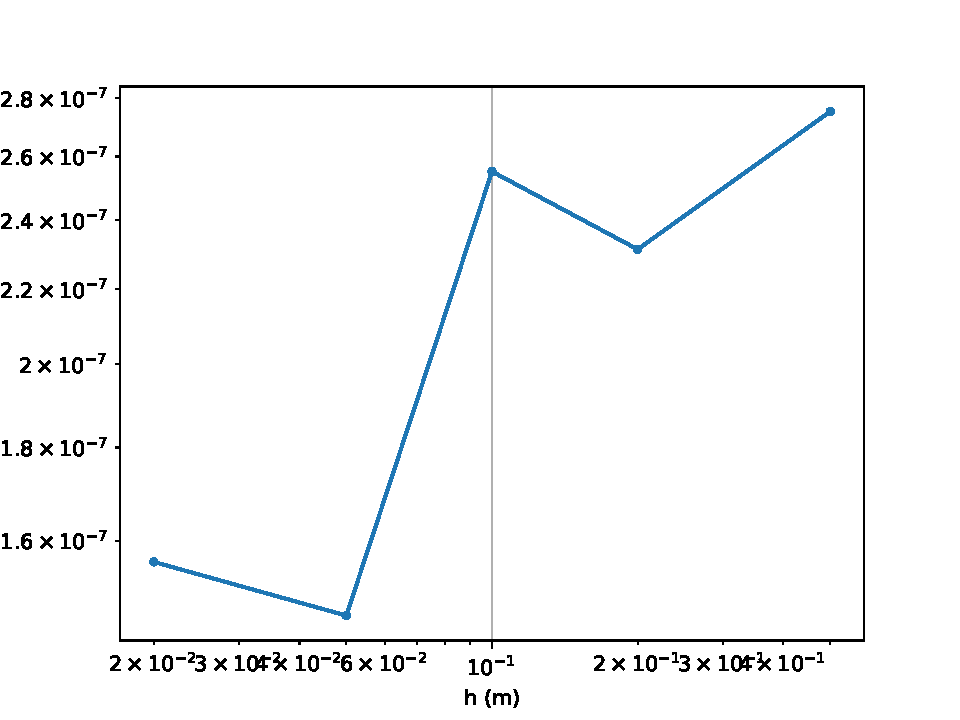
\includegraphics[width=\textwidth]{../figures/couette_err_quad_nocd_theta_0.5235987755982988_P_0.pdf}
		\caption{Convergence}
	\end{subfigure}
	\caption{Couette incliné pour P = 0 en maillage quadrilatère}
\end{figure}

\begin{figure}
	\begin{subfigure}[t]{0.3\textwidth}
		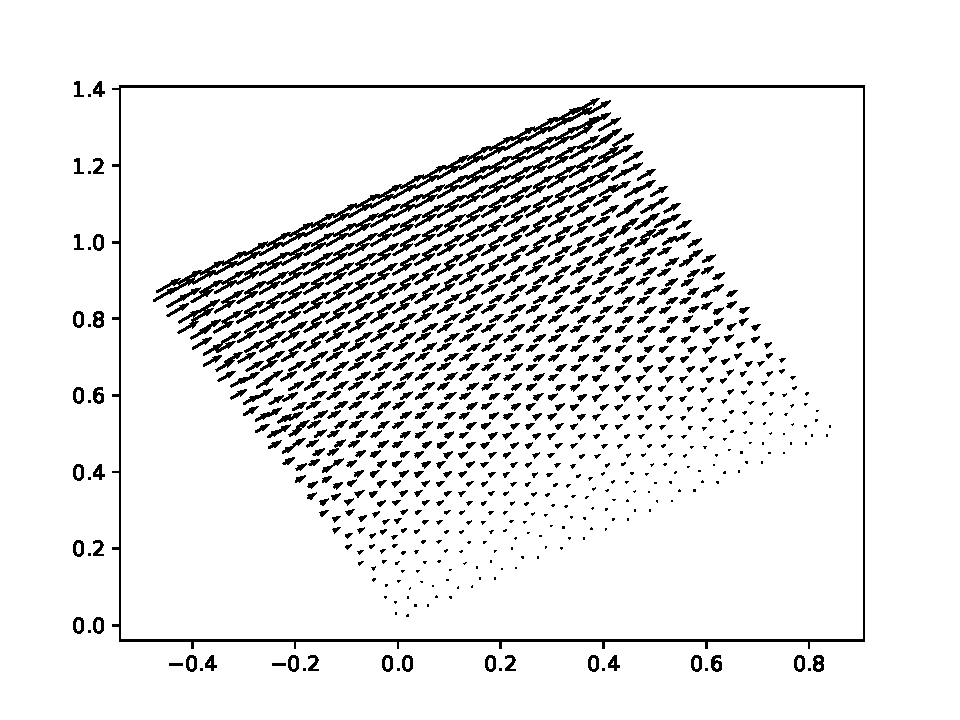
\includegraphics[width=\textwidth]{../figures/couette_vec_tri_cd_theta_0.5235987755982988_P_0.pdf}
		\caption{Champ vectoriel de vitesses}
	\end{subfigure}
	\hfill
	\begin{subfigure}[t]{0.3\textwidth}
		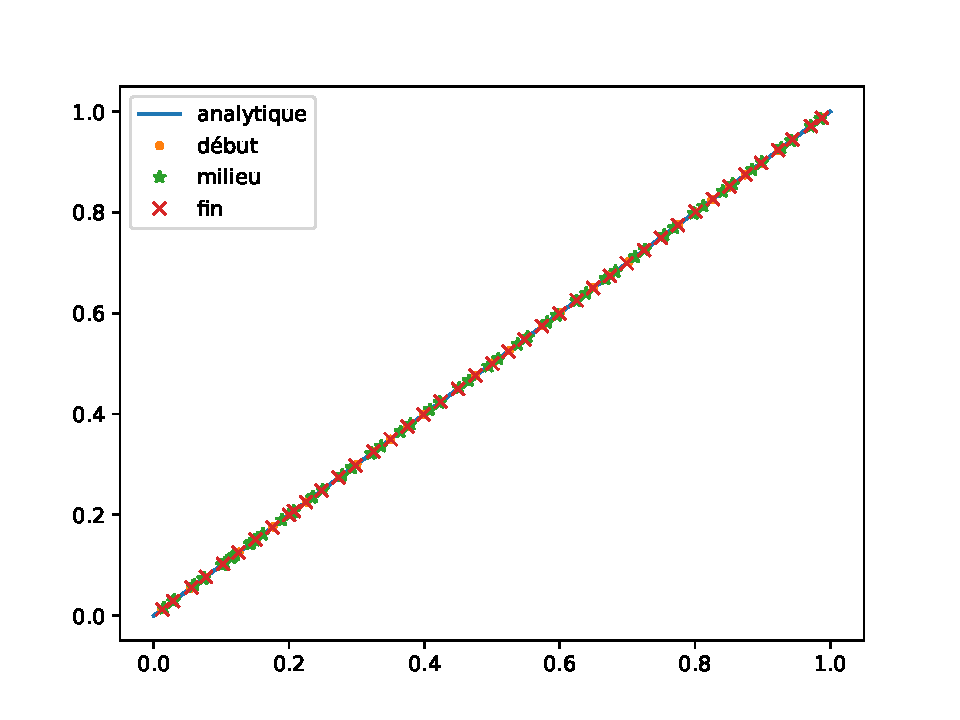
\includegraphics[width=\textwidth]{../figures/couette_slice_tri_cd_theta_0.5235987755982988_P_0.pdf}
		\caption{Slices de la solution numérique vs solution analytique}
	\end{subfigure}
	\hfill
	\begin{subfigure}[t]{0.3\textwidth}
		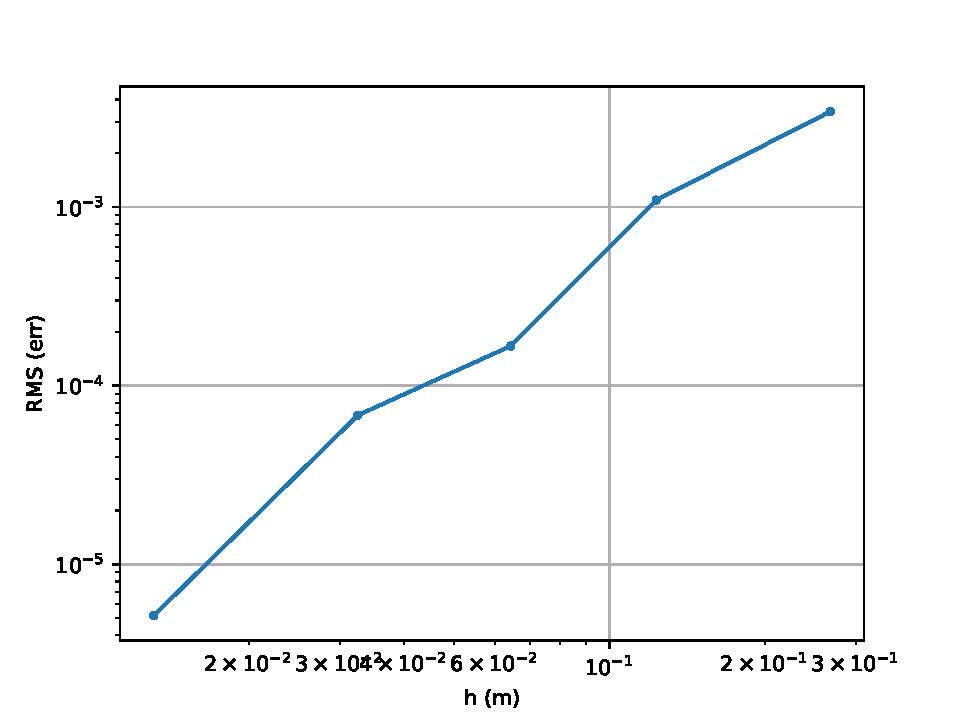
\includegraphics[width=\textwidth]{../figures/couette_err_tri_cd_theta_0.5235987755982988_P_0.pdf}
		\caption{Convergence}
	\end{subfigure}
	\caption{Couette incliné pour P = 0 en maillage triangulaire}
\end{figure}

\begin{figure}
	\begin{subfigure}[t]{0.3\textwidth}
		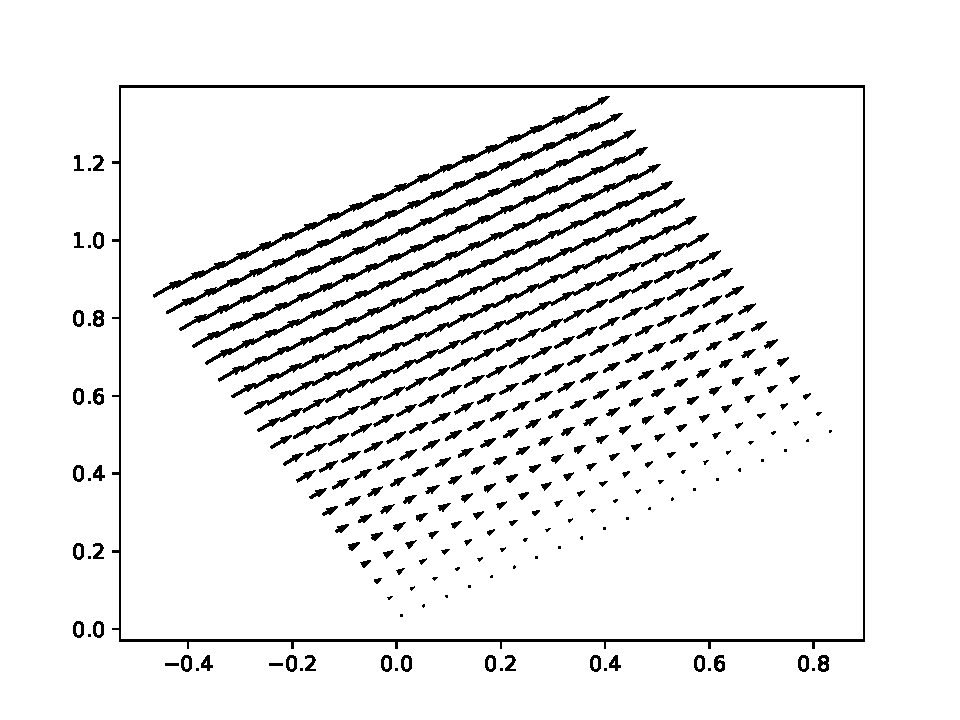
\includegraphics[width=\textwidth]{../figures/couette_vec_quad_nocd_theta_0.5235987755982988_P_1.pdf}
		\caption{Champ vectoriel de vitesses}
	\end{subfigure}
	\hfill
	\begin{subfigure}[t]{0.3\textwidth}
		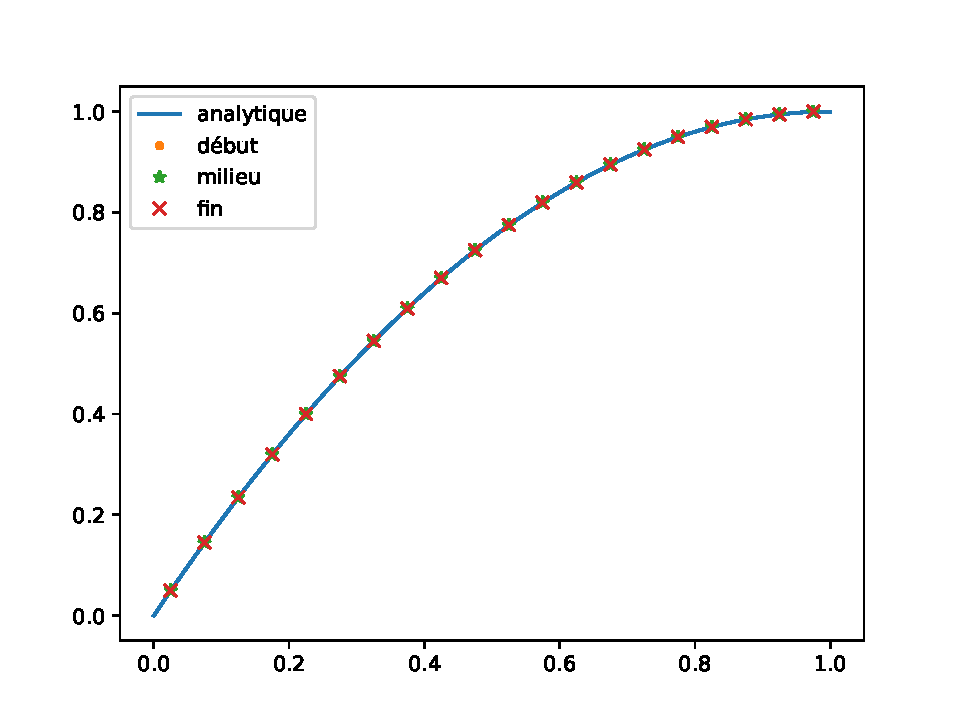
\includegraphics[width=\textwidth]{../figures/couette_slice_quad_nocd_theta_0.5235987755982988_P_1.pdf}
		\caption{Slices de la solution numérique vs solution analytique}
	\end{subfigure}
	\hfill
	\begin{subfigure}[t]{0.3\textwidth}
		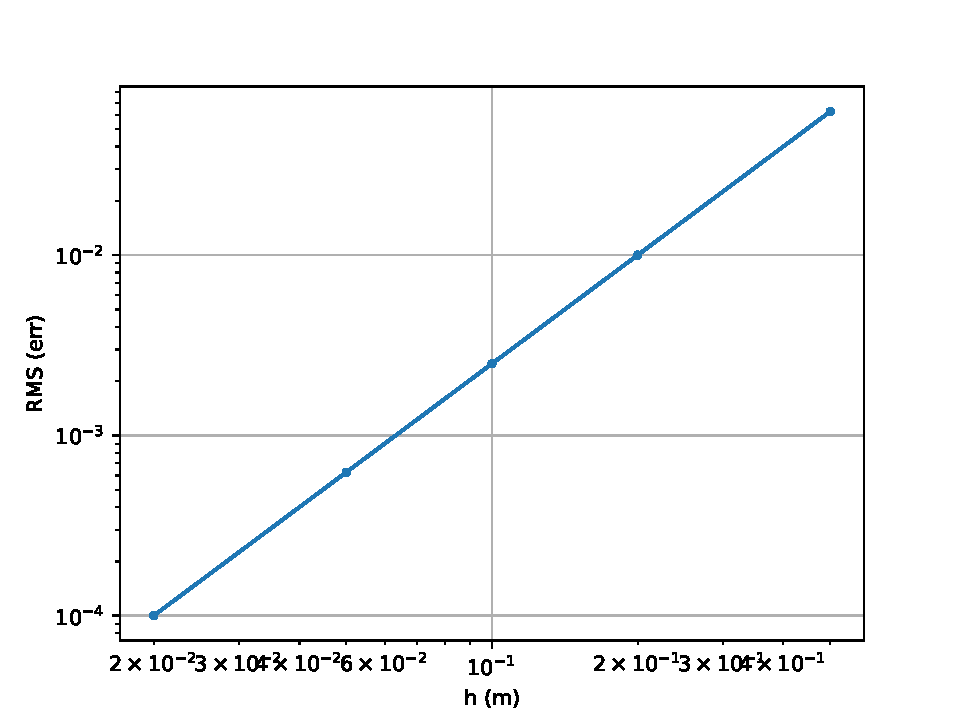
\includegraphics[width=\textwidth]{../figures/couette_err_quad_nocd_theta_0.5235987755982988_P_1.pdf}
		\caption{Convergence}
	\end{subfigure}
	\caption{Couette incliné pour P = 1 en maillage quadrilatère}
\end{figure}

\begin{figure}
	\begin{subfigure}[t]{0.3\textwidth}
		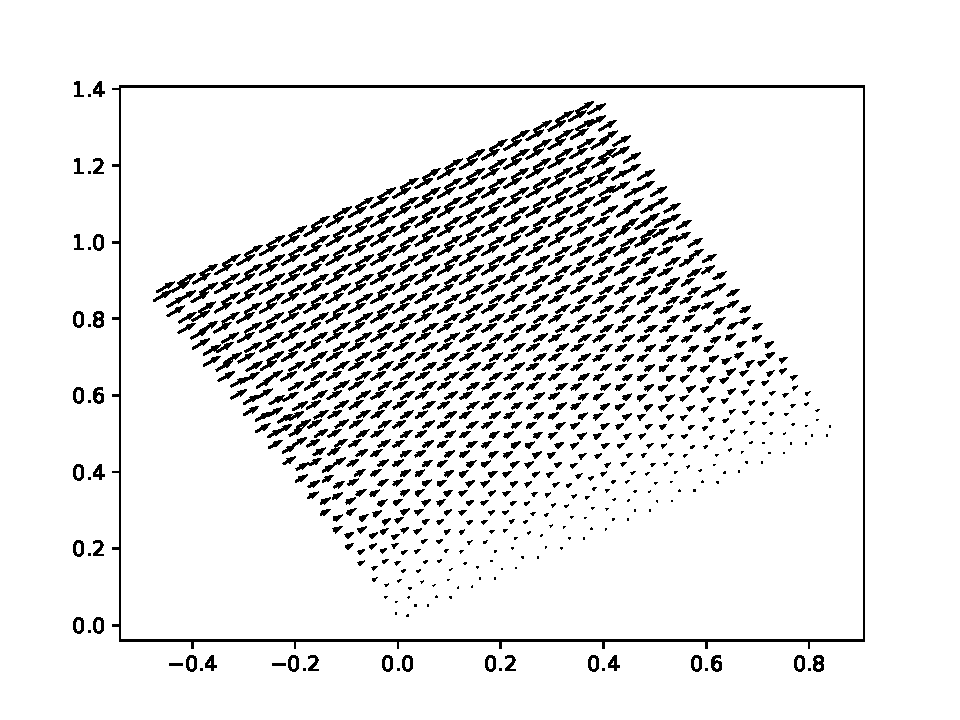
\includegraphics[width=\textwidth]{../figures/couette_vec_tri_cd_theta_0.5235987755982988_P_1.pdf}
		\caption{Champ vectoriel de vitesses}
	\end{subfigure}
	\hfill
	\begin{subfigure}[t]{0.3\textwidth}
		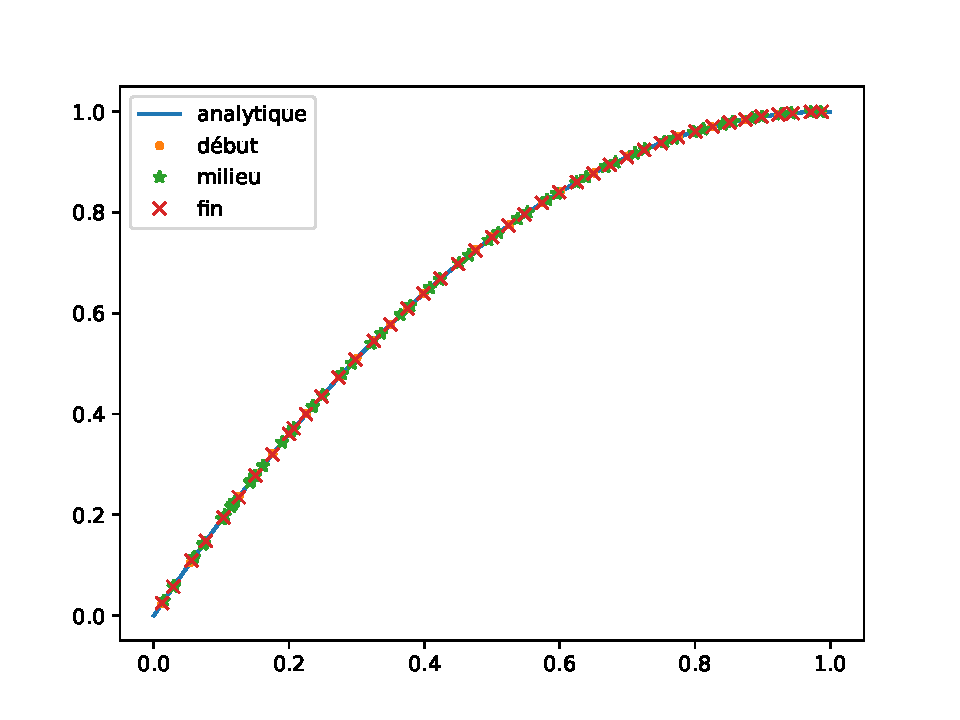
\includegraphics[width=\textwidth]{../figures/couette_slice_tri_cd_theta_0.5235987755982988_P_1.pdf}
		\caption{Slices de la solution numérique vs solution analytique}
	\end{subfigure}
	\hfill
	\begin{subfigure}[t]{0.3\textwidth}
		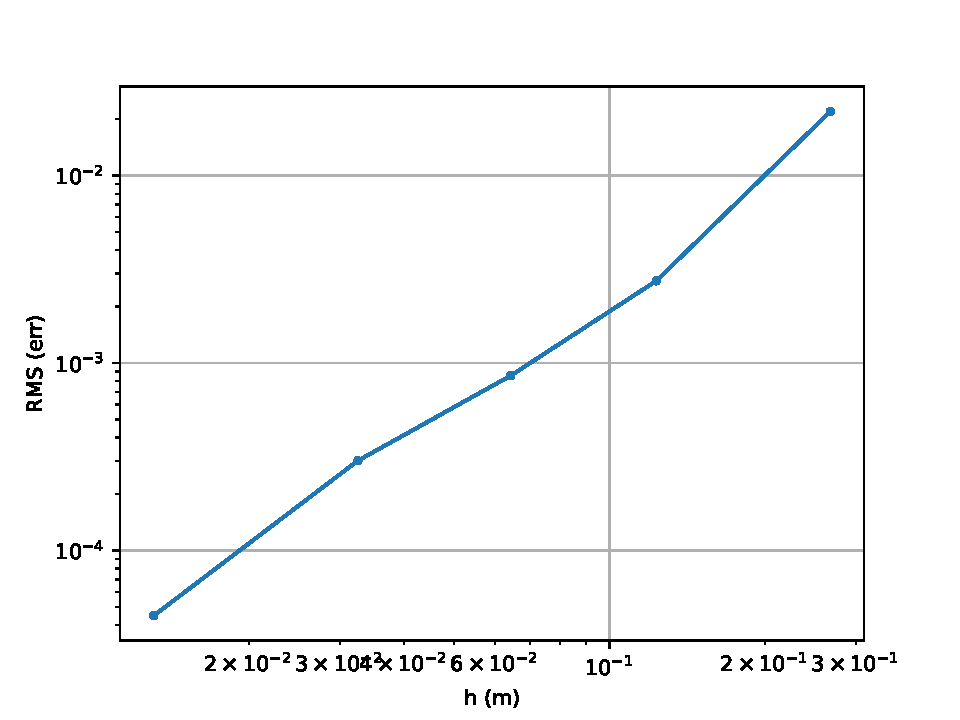
\includegraphics[width=\textwidth]{../figures/couette_err_tri_cd_theta_0.5235987755982988_P_1.pdf}
		\caption{Convergence}
	\end{subfigure}
	\caption{Couette incliné pour P = 1 en maillage triangulaire}
\end{figure}

\begin{figure}
	\begin{subfigure}[t]{0.3\textwidth}
		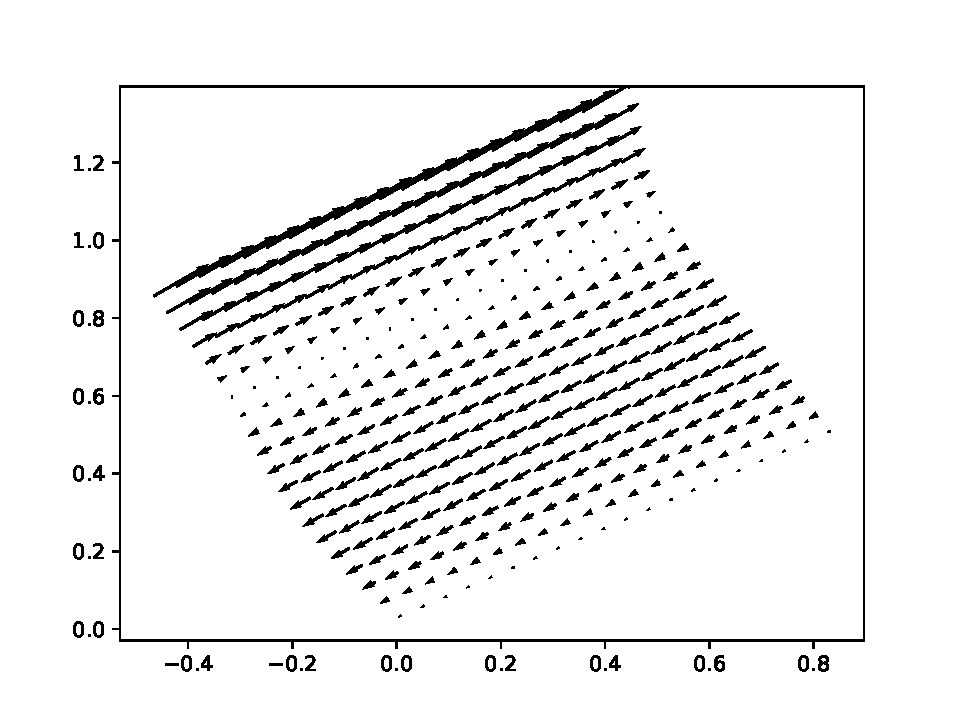
\includegraphics[width=\textwidth]{../figures/couette_vec_quad_nocd_theta_0.5235987755982988_P_-3.pdf}
		\caption{Champ vectoriel de vitesses}
	\end{subfigure}
	\hfill
	\begin{subfigure}[t]{0.3\textwidth}
		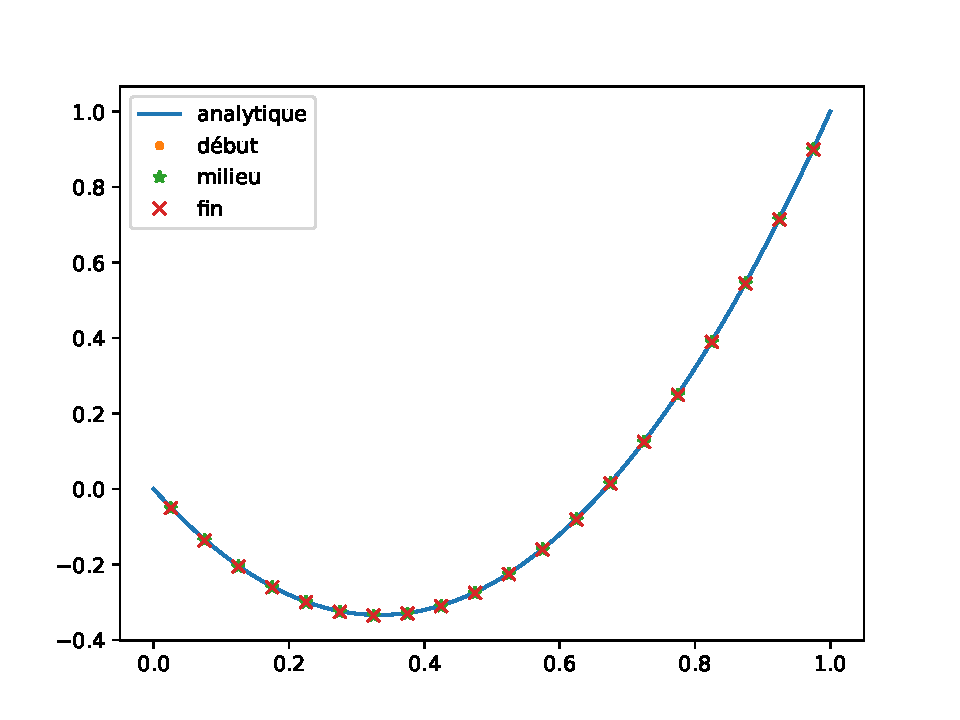
\includegraphics[width=\textwidth]{../figures/couette_slice_quad_nocd_theta_0.5235987755982988_P_-3.pdf}
		\caption{Slices de la solution numérique vs solution analytique}
	\end{subfigure}
	\hfill
	\begin{subfigure}[t]{0.3\textwidth}
		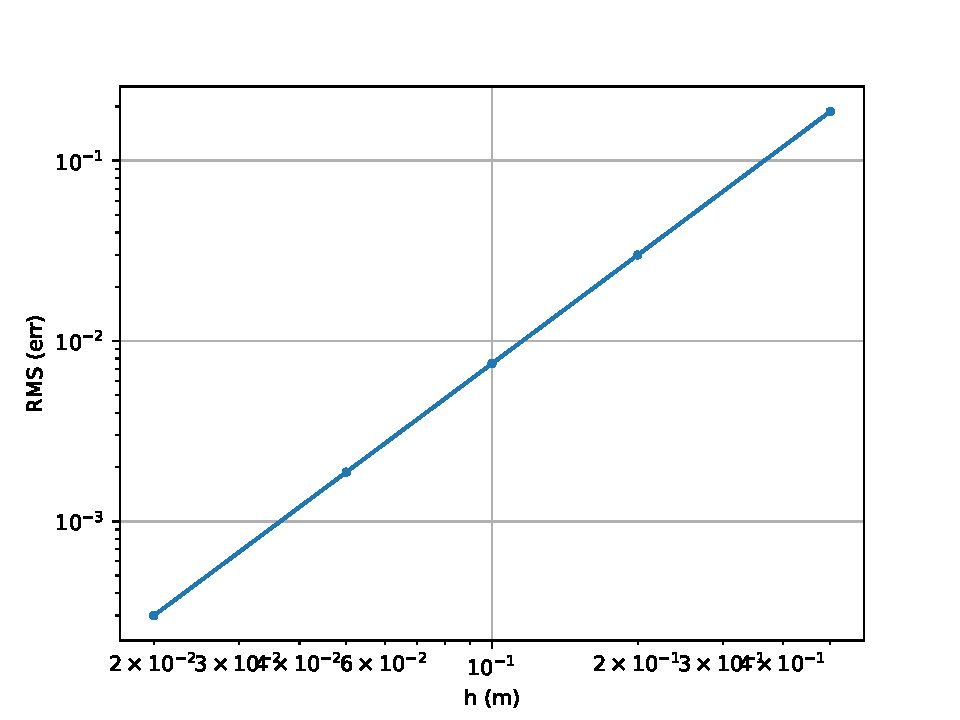
\includegraphics[width=\textwidth]{../figures/couette_err_quad_nocd_theta_0.5235987755982988_P_-3.pdf}
		\caption{Convergence}
	\end{subfigure}
	\caption{Couette incliné pour P = -3 en maillage quadrilatère}
\end{figure}

\begin{figure}
	\begin{subfigure}[t]{0.3\textwidth}
		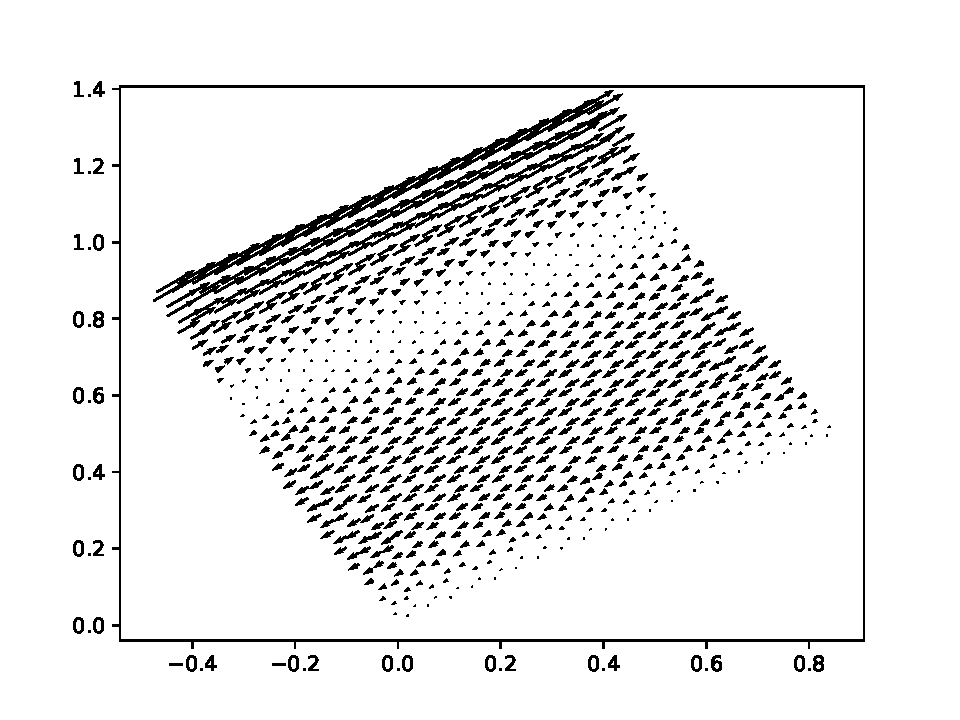
\includegraphics[width=\textwidth]{../figures/couette_vec_tri_cd_theta_0.5235987755982988_P_-3.pdf}
		\caption{Champ vectoriel de vitesses}
	\end{subfigure}
	\hfill
	\begin{subfigure}[t]{0.3\textwidth}
		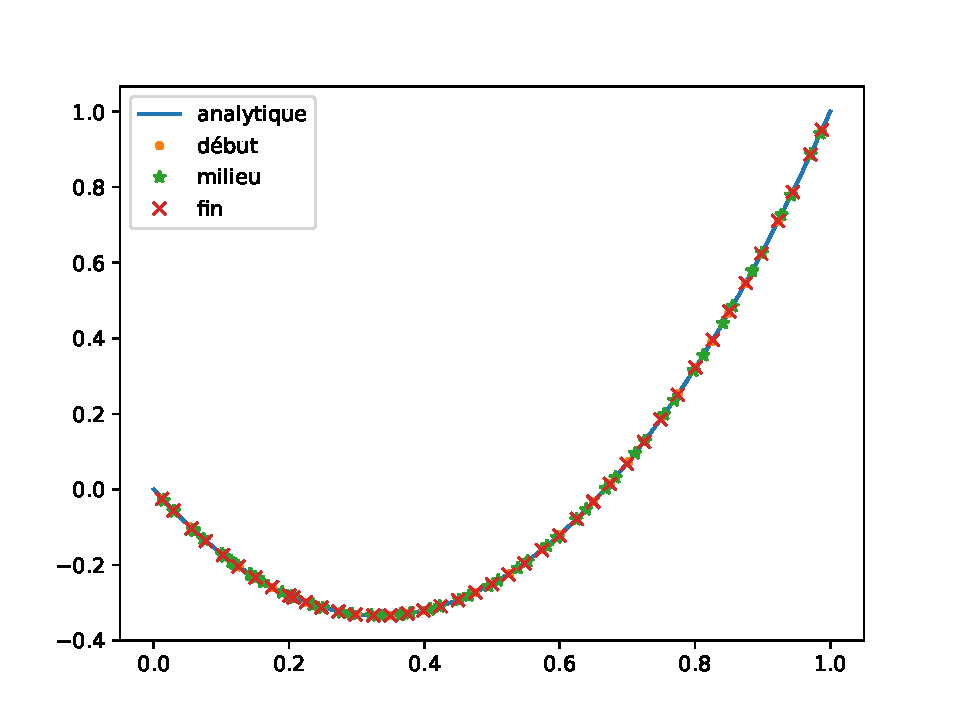
\includegraphics[width=\textwidth]{../figures/couette_slice_tri_cd_theta_0.5235987755982988_P_-3.pdf}
		\caption{Slices de la solution numérique vs solution analytique}
	\end{subfigure}
	\hfill
	\begin{subfigure}[t]{0.3\textwidth}
		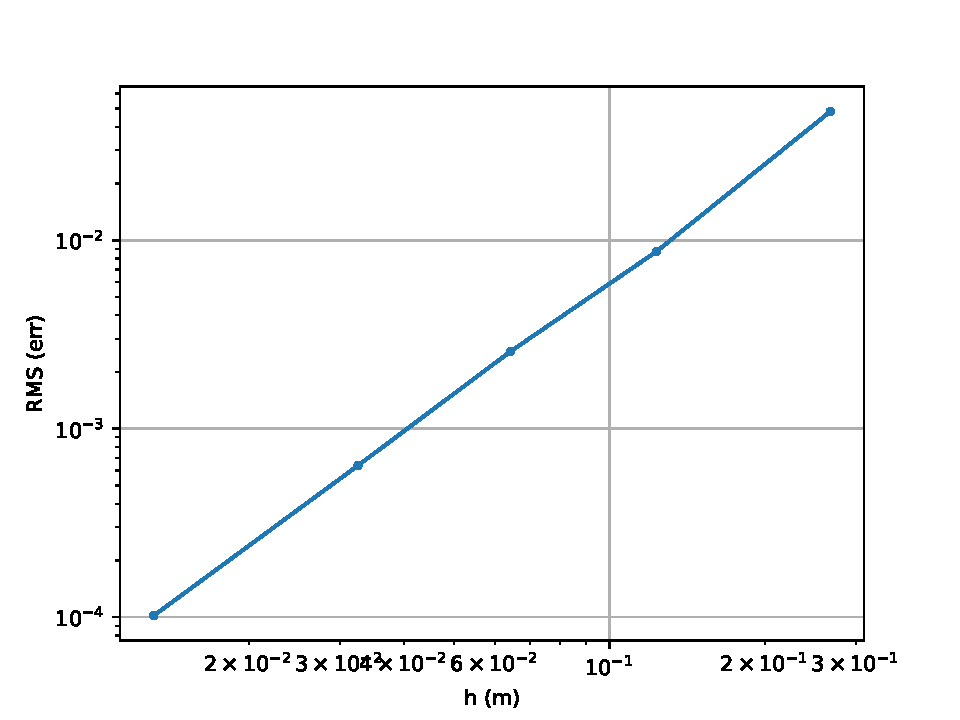
\includegraphics[width=\textwidth]{../figures/couette_err_tri_cd_theta_0.5235987755982988_P_-3.pdf}
		\caption{Convergence}
	\end{subfigure}
	\caption{Couette incliné pour P = -1 en maillage triangulaire}
\end{figure}

\printbibliography[]
	

\end{document}
